\chapter{基本使用}

	\section{常用的格式}

		\subsection{基本的段落}
			空行可以自然分隔段落:

			可以设定字体为\textit{斜体};给文字加上\underline{下划线}。可以设定字体为\textit{斜体};给文字加上\underline{下划线}。可以设定字体为\textit{斜体};给文字加上\underline{下划线}。可以设定字体为\textit{斜体};给文字加上\underline{下划线}。

			可以设定字体为\textit{斜体};给文字加上\underline{下划线}。可以设定字体为\textit{斜体};给文字加上\underline{下划线}。可以设定字体为\textit{斜体};给文字加上\underline{下划线}。可以设定字体为\textit{斜体};给文字加上\underline{下划线}。

			可以设定字体为\textit{斜体};给文字加上\underline{下划线}。可以设定字体为\textit{斜体};给文字加上\underline{下划线}。可以设定字体为\textit{斜体};给文字加上\underline{下划线}。可以设定字体为\textit{斜体};给文字加上\underline{下划线}。

		\subsection{原文照排}
			在正文中放入源文照排:在Linux下通过\verb|ls -al|查看当前目录下所有文件。

			多行的原文照排要用到verbatim环境:
			\begin{verbatim}
				/* 输出10行"Hello, world!"的面试题 */
				/* 某位童鞋的答案是这样写的        */
				printf("Hello, world!");
				printf("Hello, world!");
				printf("Hello, world!");
				printf("Hello, world!");
				printf("Hello, world!");
				printf("Hello, world!");
				printf("Hello, world!");
				printf("Hello, world!");
				printf("Hello, world!");
				printf("Hello, world!");
			\end{verbatim}

			原文照排时强调空格到verbatim*环境:
			\begin{verbatim*}
				printf("Hello, world!");
			\end{verbatim*}

		\subsection{程序代码}

			使用listings宏包的效果:

\begin{lstlisting}[language=C]
#include <stdio.h>

int main(int argc, char ** argv)
{
	printf("Hello world!\n");
	/** 看起来直接用listings和xelatex配合显示中文没有问题 **/
	printf("显示中文!\n");
	return 0;
}
\end{lstlisting}

			可以只引用整个代码中的一部分:

\begin{lstlisting}[language=C,firstline=3,lastline=9]
#include <stdio.h>

int main(int argc, char ** argv)
{
	printf("Hello world!\n");
	/** 看起来直接用listings和xelatex配合显示中文没有问题s1l1O0O0 **/
	printf("显示中文!\n");
	return 0;
}
\end{lstlisting}

			使用\verb|\lstinputlisting|引用外部文件:

			\lstinputlisting[language=HTML,firstline=2,lastline=8]{src/aa.html}

		\subsection{边注与脚注}
			按照国际惯例,这里是鬼扯的部分。\footnote{我才不承认这是为了骗稿费呢~}

			同样也给内容加上连注。但边注是没有编号的,因为就在旁边。\marginpar{这里是边注的内容。}

		\subsection{插入图片}

			试试使用浮动环境插入图片,但是这样图片就不知道浮动到什么地方去了:

			\begin{figure}[htbp]                        % 
				\centering                              % 图片居中	
				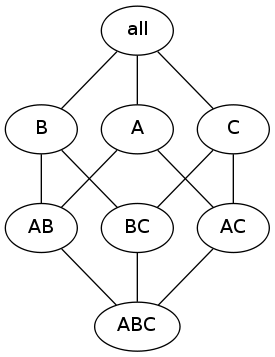
\includegraphics[scale=0.5]{dm0201.png} % scale指定缩放
				\caption{图片标题}            % 图片的标题,会自动编号
				\label{dm0201}                % 图片的标记,一定要加在caption后面。不然指向的是前一个插图
			\end{figure}

			试试使用浮动环境插入图片,但是这样图片就不知道浮动到什么地方去了:

			\begin{figure}[htbp]                        % 
				\centering                              % 图片居中	
				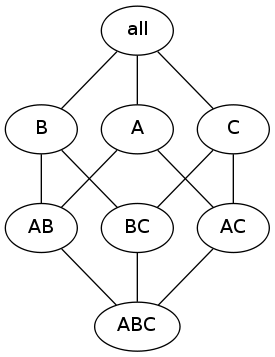
\includegraphics[scale=0.5]{dm0201.png} % scale指定缩放
				\caption{图片标题}            % 图片的标题,会自动编号
				\label{dm0202}                % 图片的标记,一定要加在caption后面。不然指向的是前一个插图
			\end{figure}

			试试使用浮动环境插入图片,但是这样图片就不知道浮动到什么地方去了:

			\begin{figure}[htbp]                        % 
				\centering                              % 图片居中	
				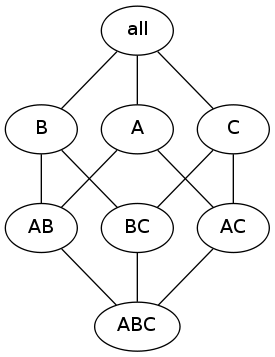
\includegraphics[scale=0.5]{dm0201.png} % scale指定缩放
				\caption{图片标题}            % 图片的标题,会自动编号
				\label{dm0203}                % 图片的标记,一定要加在caption后面。不然指向的是前一个插图
			\end{figure}


	\section{第二节}

		\subsection{第一小节}

		\subsection{第二小节}
